\documentclass[10pt]{beamer}
\usetheme[
%%% option passed to the outer theme
%    progressstyle=fixedCircCnt,   % fixedCircCnt, movingCircCnt (moving is deault)
  ]{Berlin}
  
% If you want to change the colors of the various elements in the theme, edit and uncomment the following lines

% Change the bar colors:
%\setbeamercolor{Feather}{fg=red!20,bg=red}

% Change the color of the structural elements:
%\setbeamercolor{structure}{fg=red}

% Change the frame title text color:
%\setbeamercolor{frametitle}{fg=blue}

% Change the normal text color background:
%\setbeamercolor{normal text}{fg=black,bg=gray!10}

%-------------------------------------------------------
% INCLUDE PACKAGES
%-------------------------------------------------------

\usepackage[utf8]{inputenc}
\usepackage[english]{babel}
\usepackage[T1]{fontenc}
\usepackage{amsmath}
\usepackage{helvet}
\usepackage{multirow}
\usepackage{graphicx}
\usepackage{comment}
\usepackage[absolute,overlay]{textpos}
\usepackage{tikz}
\usetikzlibrary{arrows,automata,positioning}
\usetikzlibrary{shapes.multipart}
\usetikzlibrary{decorations.markings}
\usetikzlibrary{decorations.pathreplacing}

%-------------------------------------------------------
% DEFFINING AND REDEFINING COMMANDS
%-------------------------------------------------------

% colored hyperlinks
%\renewcommand*{\Footnotemark}[1]{\NCC@makefnmark{#1}}
\newcommand{\chref}[2]{
  \href{#1}{{\usebeamercolor[bg]{Feather}#2}}
}
\newcommand{\tuple}[1]{{\langle #1 \rangle}}
\newcommand{\pre}{\mathsf{pre}}     % precondition
\newcommand{\eff}{\mathsf{eff}}     % effect
\newcommand{\cond}{\mathsf{cond}}   % conditional effect

\newcommand{\X}{\mathcal{X}}
\newcommand{\F}{\mathcal{F}}
\newcommand{\A}{\mathcal{A}}
\newcommand{\N}{\mathcal{N}}
\newcommand{\I}{\mathcal{I}}
\newcommand{\real}{\mathbb{R}}
\newcommand{\Dw}{\mathcal{D}}
\newcommand{\Xw}{\mathcal{X}}
\newcommand{\Aw}{\mathcal{A}}
\newcommand{\Rw}{\mathcal{R}}
\newcommand{\OO}{\mathcal{O}}
\newcommand{\tOO}{\wt{\OO}}
\newcommand{\II}[1]{\mathbb{I}{\left\{#1\right\}}}
\newcommand{\PP}[1]{\mathbb{P}\left[#1\right]}
\newcommand{\EE}[1]{\mathbb{E}\left[#1\right]}
\newcommand{\EEs}[2]{\mathbb{E}_{#2}\left[#1\right]}
\newcommand{\PPt}[1]{\mathbb{P}_t\left[#1\right]}
\newcommand{\EEt}[1]{\mathbb{E}_t\left[#1\right]}
\newcommand{\PPi}[1]{\mathbb{P}_i\left[#1\right]}
\newcommand{\EEi}[1]{\mathbb{E}_i\left[#1\right]}
\newcommand{\EEp}[1]{\mathbb{E}_{\pi,P}\left[#1\right]}
\newcommand{\EEcp}[2]{\mathbb{E}_{\pi,P}\left[\left.#1\right|#2\right]}
\newcommand{\PPc}[2]{\mathbb{P}\left[#1\left|#2\right.\right]}
\newcommand{\PPct}[2]{\mathbb{P}_t\left[#1\left|#2\right.\right]}
\newcommand{\PPcc}[2]{\mathbb{P}\left[\left.#1\right|#2\right]}
\newcommand{\PPcct}[2]{\mathbb{P}_t\left[\left.#1\right|#2\right]}
\newcommand{\PPcci}[2]{\mathbb{P}_i\left[\left.#1\right|#2\right]}
\newcommand{\EEc}[2]{\mathbb{E}\left[#1\left|#2\right.\right]}
\newcommand{\EEcc}[2]{\mathbb{E}\left[\left.#1\right|#2\right]}
\newcommand{\EEcs}[3]{\mathbb{E}_{#3}\left[\left.#1\right|#2\right]}
\newcommand{\EEcct}[2]{\mathbb{E}_t\left[\left.#1\right|#2\right]}
\newcommand{\EEcci}[2]{\mathbb{E}_i\left[\left.#1\right|#2\right]}
\renewcommand{\th}{\ensuremath{^{\mathrm{th}}}}
\def\argmin{\mathop{\mbox{ arg\,min}}}
\def\argmax{\mathop{\mbox{ arg\,max}}}
\newcommand{\ra}{\rightarrow}

\newcommand{\norm}[1]{\left\|#1\right\|}
\newcommand{\onenorm}[1]{\norm{#1}_1}
\newcommand{\infnorm}[1]{\norm{#1}_\infty}
\newcommand{\iprod}[2]{\left\langle#1,#2\right\rangle}
\newcommand{\ev}[1]{\left\{#1\right\}}
\newcommand{\pa}[1]{\left(#1\right)}
\newcommand{\bpa}[1]{\bigl(#1\bigr)}
\newcommand{\Bpa}[1]{\Bigl(#1\Bigr)}
\newcommand{\sign}{\mbox{sign}}
\newcommand{\wh}{\widehat}
\newcommand{\wt}{\widetilde}
\newcommand{\transpose}{^\top}

\newcommand{\loss}{\ell}
\newcommand{\hloss}{\wh{\loss}}
\newcommand{\hL}{\wh{L}}
\newcommand{\tZ}{\wt{Z}}
\newcommand{\reg}{\mathfrak{R}}
\newcommand{\hreg}{\widehat{\reg}}
\newcommand{\hr}{\wh{r}}
\newcommand{\hv}{\wh{v}}
\newcommand{\hq}{\wh{q}}
\newcommand{\hmu}{\wh{\mu}}
\newcommand{\hR}{\wh{R}}
\newcommand{\tmu}{\wt{\mu}}
\newcommand{\tN}{\wt{N}}
\newcommand{\RE}[2]{\mbox{RE}\left(\left.#1\right\|#2\right)}
\newcommand{\KL}[2]{\mbox{KL}\left(#1\middle\lVert#2\right)}
\newcommand{\DD}[3]{D_{#3}\left(#1\middle\lVert#2\right)}
\newcommand{\DDC}[2]{\DD{#1}{#2}{C}}
\newcommand{\DDS}[2]{\DD{#1}{#2}{S}}

\newcommand{\trho}{\wt{\rho}}

\definecolor{gold}{rgb}{1,0.75,0}
\definecolor{darkred}{rgb}{0.75,0,0}
\setbeamercolor*{goldc}{fg=black,bg=gold}
\definecolor{darkpurp}{rgb}{0.4,0.2,0.4}
\setbeamercolor*{purpc}{fg=white,bg=darkpurp}
\setbeamercolor*{redc}{fg=white,bg=darkred}
\newcommand{\hG}[1]{\large \textcolor{darkred}{#1}}

\newcommand{\redd}[1]{\textcolor{darkred}{#1}}
\newcommand{\goldd}[1]{\textcolor{gold}{#1}}

\definecolor{ballblue}{rgb}{0.0, 0.53, 0.74}
\definecolor{lightgray}{rgb}{0.85, 0.85, 0.85}

%-------------------------------------------------------
% INFORMATION IN THE TITLE PAGE
%-------------------------------------------------------

\title[] % [] is optional - is placed on the bottom of the sidebar on every slide
{ % is placed on the title page
      \textbf{Machine Learning}
}

\author[Jonsson \& G\'omez]
{      Anders Jonsson \& Vicen\c{c} G\'omez \\
\vspace*{0.5cm}
Master in Intelligence Interactive Systems\\
2020-21\\
\vspace*{0.5cm}
Lecture 4\\
Optimization and Gradient Descent
%      {\ttfamily bagchi.bhaskar@cse.iitkgp.ernet.in}
}

\date{}

\AtBeginSection[]
{
   \begin{frame}
       \frametitle{Content}
       \tableofcontents[currentsection]
   \end{frame}
}

%-------------------------------------------------------
% THE BODY OF THE PRESENTATION
%-------------------------------------------------------

\begin{document}

%-------------------------------------------------------
% THE TITLEPAGE
%-------------------------------------------------------

\begin{frame}[plain,noframenumbering] % the plain option removes the header from the title page, noframenumbering removes the numbering of this frame only
  \titlepage % call the title page information from above
\end{frame}

\begin{frame}{Content}{}
\tableofcontents
\end{frame}

\section{Optimization}

\begin{frame}
  \frametitle{Empirical risk minimization}
  \begin{itemize}
	\item Find the hypothesis $h\in\mathcal{H}$ that minimizes the empirical risk $L_S(h)$
	\item Fundamentally, this is a problem of {\color{blue} optimization}
	\item Supervised learning is {\color{red} intrinsically linked} to optimization
  \end{itemize}
  \begin{center}
  \includegraphics[height=5cm]{images/optimization.jpg}
  \end{center}
\end{frame}

\begin{frame}
  \frametitle{Properties of functions}
  \begin{center}
  \begin{tabular}{ccc}
  \includegraphics[height=2.5cm]{images/continuum.png} & \includegraphics[height=2.5cm]{images/convexfun.png} & \includegraphics[height=2.5cm]{images/smooth.png}\\
  (Non-)Differentiable & Convex & Smooth
  \end{tabular}
  \end{center}
\end{frame}

\begin{frame}
  \frametitle{Differentiable function}
  \begin{center}
  \begin{tabular}{c@{\hspace*{1cm}}c}
  \includegraphics[height=2.5cm]{images/continuum.png} & \includegraphics[height=2.5cm]{images/nondiff.png}
  \end{tabular}
  \end{center}
  \begin{itemize}
	\item A function $f:C\rightarrow\mathbb{R}$ is {\color{red} differentiable} if it is continuous and has a finite gradient in each point $x\in C$
	\item For continuous functions, we can still compute a {\color{blue} sub-gradient}
  \end{itemize}
\end{frame}

\begin{frame}
  \frametitle{Convex set}
  \begin{center}
  \includegraphics[height=2.5cm]{images/convex.png}
  \end{center}
  \begin{definition}
	A set $C$ is {\color{red} convex} if, for any two points $x_1,x_2\in C$, the entire line segment between $x_1$ and $x_2$ is also in $C$. Formally, for any $\alpha\in[0,1]$, \[\alpha x_1 + (1-\alpha)x_2 \in C\]
  \end{definition}
\end{frame}

\begin{frame}
  \frametitle{Convex function}
  \begin{center}
  \includegraphics[height=4cm]{images/convexfun.png}
  \end{center}
  \begin{definition}
	Let $C$ be a convex set. A function $f:C\rightarrow\mathbb{R}$ is {\color{red} convex} if, for any $x_1,x_2\in C$ and $\alpha\in[0,1]$, $f(\alpha x_1 + (1-\alpha)x_2) \leq \alpha f(x_1) + (1-\alpha) f(x_2)$
  \end{definition}
\end{frame}

\begin{frame}
  \frametitle{Local minimum}
  \begin{center}
  \includegraphics[height=3cm]{images/minimum.png}
  \end{center}
  Given $x\in C$ and $\delta\in\mathbb{R}$, let $B(x,\delta)=\{y \in C:\lVert y-x\rVert\leq \delta\}$ be a ball of radius $\delta$ around $x$
  \begin{definition}
	Given a function $f:C\rightarrow\mathbb{R}$, an element $x_0\in C$ is a {\color{red} local minimum} if there exists $\delta\in\mathbb{R}$ such that for each $x\in B(x_0,\delta)$, $f(x_0)\leq f(x)$
  \end{definition}
\end{frame}

\begin{frame}
  \frametitle{Global minimum}
  \begin{center}
  \includegraphics[height=4cm]{images/convexfun.png}
  \end{center}
  \begin{theorem}
	Every local minimum of a convex function $f:C\rightarrow\mathbb{R}$ is also global.
  \end{theorem}
\end{frame}

\begin{frame}
  \frametitle{Tangent}
  \begin{center}
  \includegraphics[height=4cm]{images/tangent.png}
  \end{center}
  Tangent at $x_0\in C$: linear function $l(x) = f(x_0) + \langle \nabla f(x_0), x - x_0 \rangle$
  \begin{theorem}
	Given a convex function $f:C\rightarrow\mathbb{R}$, the tangent at any point $x_0\in C$ lies below $f$, i.e.~for each $x\in C$, $f(x_0) + \langle \nabla f(x_0), x - x_0 \rangle \leq f(x)$
  \end{theorem}
\end{frame}

\begin{frame}
  \frametitle{Convexity}
  \begin{center}
  \includegraphics[height=4cm]{images/convexfun.png}
  \end{center}
  For a {\color{red} univariate}, twice differentiable function $f:C\rightarrow\mathbb{R}$, the following statements are equivalent:
  \begin{itemize}
	\item $f$ is convex
	\item $f'$ is monotonically non-decreasing
	\item $f''$ is non-negative
  \end{itemize}
\end{frame}

\begin{frame}
  \frametitle{Smoothness}
  \begin{center}
  \includegraphics[height=4cm]{images/smooth.png}
  \end{center}
  \vspace*{-2cm}
  \begin{definition}
	A differentiable function $f:C\rightarrow\mathbb{R}$ is {\color{red} $\beta$-smooth} if, for each $x_1,x_2\in C$, $\lVert \nabla f(x_2) - \nabla f(x_1) \rVert \leq \beta \lVert x_2 - x_1 \rVert$
  \end{definition}
\end{frame}

\begin{frame}
  \frametitle{Smoothness and convexity}
  \begin{center}
  \includegraphics[height=4cm]{images/smooth.png}
  \end{center}
  \vspace*{-2cm}
  \begin{itemize}
	\item If a function $f:C\rightarrow\mathbb{R}$ is $\beta$-smooth, then for each $x_1,x_2\in C$,
	\[f(x_2) \leq f(x_1) + \langle \nabla f(x_1), x_2 - x_1 \rangle + \frac \beta 2 \lVert x_2 - x_1 \rVert^2\]
	\item If the function $f$ is also convex, we obtain
	\[0 \leq f(x_2) - f(x_1) - \langle \nabla f(x_1), x_2 - x_1 \rangle \leq \frac \beta 2 \lVert x_2 - x_1 \rVert^2\]
  \end{itemize}
  \vspace*{-.8cm}
  \begin{center}
  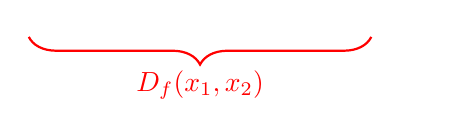
\begin{tikzpicture}
    \node at (8.8,4.9) {};
	\draw[thick,red,decorate,decoration={brace,amplitude=10pt}] (8.05,4.9) -- (3.7,4.9) node [midway,below,yshift=-.3cm] {$D_f(x_1,x_2)$};
  \end{tikzpicture}
  \end{center}
\end{frame}

\begin{frame}
  \frametitle{Convex learning problem}
  \begin{itemize}
	\item Consider a supervised learning problem $\langle \mathcal{X},\mathcal{D},\mathcal{Y},f,S\rangle$
	\item The learner chooses $\langle \mathcal{H}, \ell, \mathcal{A} \rangle$
	\item The learning problem is {\color{red} convex} if the following holds:
	\begin{enumerate}
	\item The hypothesis class $\mathcal{H}$ is a {\color{red} convex set}
	\item The loss $\ell$ and empirical risk $L_S:\mathcal{H}\rightarrow\mathbb{R}$ are {\color{red} convex functions}
	\end{enumerate}
  \end{itemize}
\end{frame}

\begin{frame}
  \frametitle{Recipe for loss functions}
  Given convex functions $f$ and $g$, the following functions are all convex:
  \begin{enumerate}
	\item All norms.
	\item $h(x) = a\cdot f(x)$, for any constant $a>0$.
	\item $h(x) = f(x) + g(x)$.
	\item $h(x) = \max(f(x),g(x))$.
	\item $h(x) = f(Ax + b)$, for any $d\times d$ matrix $A$ and $d\times 1$ vector $b$.
  \end{enumerate}
\end{frame}

\begin{frame}
  \frametitle{Learnability of convex learning problems}
  \begin{itemize}
	\item For any algorithm $\mathcal{A}$, there are convex learning problems on which it fails
	\item This holds even if $\mathcal{H}$ is bounded (e.g.~$\lVert w\rVert \leq B$)
	\item However, if the loss function is also $\beta$-smooth, then the convex learning problem is learnable
	\item Learnability conditions: {\color{red} convex} + {\color{blue} bounded} + {\color{green} smooth}
  \end{itemize}
\end{frame}

\begin{frame}
  \frametitle{Surrogate loss}
  \begin{center}
  \includegraphics[height=5cm]{images/losses.png}
  \end{center}
  \begin{itemize}
	\item If a learning problem is non-convex, we can {\color{red} approximate} it using a convex loss function that {\color{blue} upper bounds} the original loss
	\item Example: 0-1 loss
  \end{itemize}
\end{frame}

\section{Gradient descent}

\begin{frame}
  \frametitle{Gradient descent}
  \begin{center}
  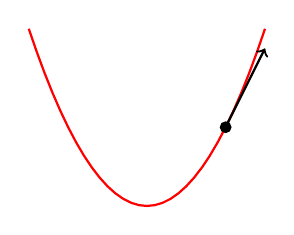
\begin{tikzpicture}
  \draw[thick,red] plot [smooth] (0.5,2.25) -- (0.6,1.96) -- (0.7,1.69) -- (0.8,1.44) -- (0.9,1.21) -- (1,1) -- (1.1,0.81) -- (1.2,0.64) -- (1.3,0.49) -- (1.4,0.36) -- (1.5,0.25) -- (1.6,0.16) -- (1.7,0.09) -- (1.8,0.04) -- (1.9,0.01) -- (2,0) -- (2.1,0.01) -- (2.2,0.04) -- (2.3,0.09) -- (2.4,0.16) -- (2.5,0.25) -- (2.6,0.36) -- (2.7,0.49) -- (2.8,0.64) -- (2.9,0.81) -- (3,1) -- (3.1,1.21) -- (3.2,1.44) -- (3.3,1.69) -- (3.4,1.96) -- (3.5,2.25);
  \draw[thick,fill=black] (3,1) circle (0.06cm);
  \draw[thick,->] (3,1) -- (3.5,2);
  \end{tikzpicture}
  \end{center}
  \begin{itemize}
	\item Convex, differentiable loss function $L_S$
	\item Idea: descend in the opposite direction of the {\color{red} gradient}
  \end{itemize}
\end{frame}

\begin{frame}
  \frametitle{Algorithm}
  \begin{center}
  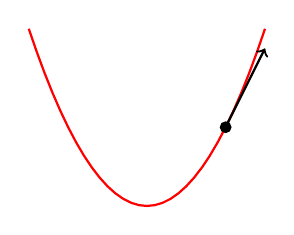
\begin{tikzpicture}
  \draw[thick,red] plot [smooth] (0.5,2.25) -- (0.6,1.96) -- (0.7,1.69) -- (0.8,1.44) -- (0.9,1.21) -- (1,1) -- (1.1,0.81) -- (1.2,0.64) -- (1.3,0.49) -- (1.4,0.36) -- (1.5,0.25) -- (1.6,0.16) -- (1.7,0.09) -- (1.8,0.04) -- (1.9,0.01) -- (2,0) -- (2.1,0.01) -- (2.2,0.04) -- (2.3,0.09) -- (2.4,0.16) -- (2.5,0.25) -- (2.6,0.36) -- (2.7,0.49) -- (2.8,0.64) -- (2.9,0.81) -- (3,1) -- (3.1,1.21) -- (3.2,1.44) -- (3.3,1.69) -- (3.4,1.96) -- (3.5,2.25);
  \draw[thick,fill=black] (3,1) circle (0.06cm);
  \draw[thick,->] (3,1) -- (3.5,2);
  \end{tikzpicture}
  \end{center}
  \begin{block}{Gradient descent}
  \begin{enumerate}
	\item Initialize weight vector $w_0=0$
	\item Compute the gradient $\nabla_w L_S(w_0)$
	\item Update weights as $w_1\leftarrow w_0 - \eta \nabla_w L_S(w_0)$
	\item Repeat from 2. for weight vector $w_t$, $t=1,2,\ldots$
  \end{enumerate}
  \end{block}
\end{frame}

\begin{frame}
  \frametitle{Learning rate}
  \begin{center}
  \includegraphics[height=4cm]{images/gradient.png}
  \end{center}
  \begin{itemize}
	\item Learning rate $\eta$ determines the rate of descent
	\item Too large: learning oscillates and may never reach minimum
	\item Too small: learning is slow and may never reach minimum
  \end{itemize}
\end{frame}

%\begin{frame}
%  \frametitle{Convergence of gradient descent}
%  Assume that the minimum is given by $w^*$
%  \begin{theorem}
%	Any algorithm with $w_0=0$ and whose update rule is on the form
%	\[w_{t+1}\leftarrow w_t - \eta v_t\]
%	satisfies 
%	\[\sum_{t=1}^T \langle w_t - w^*, v_t \rangle \leq \frac {\lVert w^* \rVert^2} 2 + \frac \eta 2 \sum_{t+1}^T \lVert v_t \rVert^2\]
%  \end{theorem}
%\end{frame}

\begin{frame}
  \frametitle{Convergence of gradient descent}
  \begin{itemize}
	\item Let $f$ be a convex and $\rho$-smooth function
	\item Let $\mathcal{H}=\{w:\lVert w\rVert \leq B\}$ and let $w^* = \arg\min_{w\in\mathcal{H}} f(w)$
	\item Run gradient descent for $T$ iterations with learning rate $\eta = \frac B {\rho\sqrt{T}}$
	\item Output the {\color{red} average} weight vector $\bar{w}=\frac 1 T \sum_{t=1}^T w_t$
  \end{itemize}
  \pause
  \begin{theorem}
	The output vector $\bar{w}$ satisfies
	\[f(\bar{w}) - f(w^*) \leq \frac {B\rho} {\sqrt{T}}\]
	For a desired accuracy $\epsilon$, the number of required iterations is
	\[T \geq \frac {B^2\rho^2} {\epsilon^2}\]
  \end{theorem}
\end{frame}

\begin{frame}
  \frametitle{Properties of gradient descent}
  \begin{itemize}
	\item Provably converges if learning problem is convex and learnable
	\item However, computing $\nabla_w L_S(w_t)$ requires iterating over $S$
	\item If the training set $S$ is large, gradient descent is {\color{red} inefficient}
  \end{itemize}
\end{frame}

\begin{frame}
  \frametitle{Stochastic gradient descent (SGD)}
  \begin{center}
  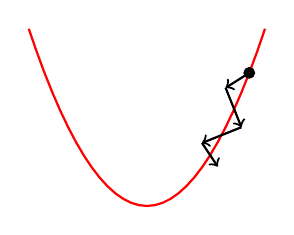
\begin{tikzpicture}
  \draw[thick,red] plot [smooth] (0.5,2.25) -- (0.6,1.96) -- (0.7,1.69) -- (0.8,1.44) -- (0.9,1.21) -- (1,1) -- (1.1,0.81) -- (1.2,0.64) -- (1.3,0.49) -- (1.4,0.36) -- (1.5,0.25) -- (1.6,0.16) -- (1.7,0.09) -- (1.8,0.04) -- (1.9,0.01) -- (2,0) -- (2.1,0.01) -- (2.2,0.04) -- (2.3,0.09) -- (2.4,0.16) -- (2.5,0.25) -- (2.6,0.36) -- (2.7,0.49) -- (2.8,0.64) -- (2.9,0.81) -- (3,1) -- (3.1,1.21) -- (3.2,1.44) -- (3.3,1.69) -- (3.4,1.96) -- (3.5,2.25);
  \draw[thick,fill=black] (3.3,1.69) circle (0.06cm);
  \draw[thick,->] (3.3,1.69) -- (3,1.5);
  \draw[thick,->] (3,1.5) -- (3.2,1);
  \draw[thick,->] (3.2,1) -- (2.7,0.8);
  \draw[thick,->] (2.7,0.8) -- (2.9,0.5);
  \end{tikzpicture}
  \end{center}
  \begin{itemize}
	\item Idea: compute {\color{blue} partial gradient} on subset of data points
	\item Each partial gradient does not coincide with the full gradient
	\item In {\color{green} expectation}, partial gradients descend towards minimum
  \end{itemize}
\end{frame}

\begin{frame}
  \frametitle{Algorithm}
  \begin{center}
  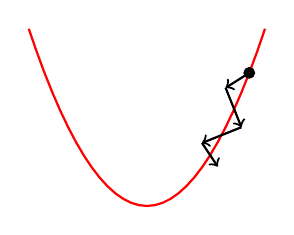
\begin{tikzpicture}
  \draw[thick,red] plot [smooth] (0.5,2.25) -- (0.6,1.96) -- (0.7,1.69) -- (0.8,1.44) -- (0.9,1.21) -- (1,1) -- (1.1,0.81) -- (1.2,0.64) -- (1.3,0.49) -- (1.4,0.36) -- (1.5,0.25) -- (1.6,0.16) -- (1.7,0.09) -- (1.8,0.04) -- (1.9,0.01) -- (2,0) -- (2.1,0.01) -- (2.2,0.04) -- (2.3,0.09) -- (2.4,0.16) -- (2.5,0.25) -- (2.6,0.36) -- (2.7,0.49) -- (2.8,0.64) -- (2.9,0.81) -- (3,1) -- (3.1,1.21) -- (3.2,1.44) -- (3.3,1.69) -- (3.4,1.96) -- (3.5,2.25);
  \draw[thick,fill=black] (3.3,1.69) circle (0.06cm);
  \draw[thick,->] (3.3,1.69) -- (3,1.5);
  \draw[thick,->] (3,1.5) -- (3.2,1);
  \draw[thick,->] (3.2,1) -- (2.7,0.8);
  \draw[thick,->] (2.7,0.8) -- (2.9,0.5);
  \end{tikzpicture}
  \end{center}
  \begin{block}{SGD}
  \begin{enumerate}
	\item Initialize weight vector $w_0=0$
	\item Compute a partial gradient $v_0$ such that $\mathbb{E}[v_0|w_0] = \nabla_w L_S(w_0)$
	\item Update weights as $w_1\leftarrow w_0 - \eta v_0$
	\item Repeat from 2. for weight vector $w_t$, $t=1,2,\ldots$
  \end{enumerate}
  \end{block}
\end{frame}

\begin{frame}
  \frametitle{Partial gradient}
  \begin{itemize}
	\item Given weight vector $w_t$, several ways to compute partial gradient:
	\begin{enumerate}
	\item Compute gradient of loss function $\ell(h(w_t,x),y)$ on {\color{red} data point $(x,y)$}
	\item Compute partial gradient on {\color{blue} mini-batch} $S'\subset S$
	\end{enumerate}
  \end{itemize}
\end{frame}

\begin{frame}
  \frametitle{Convergence of stochastic gradient descent}
  \begin{itemize}
	\item Let $f$ be a convex and $\rho$-smooth function
	\item Let $\mathcal{H}=\{w:\lVert w\rVert \leq B\}$ and let $w^* = \arg\min_{w\in\mathcal{H}} f(w)$
	\item Run SGD for $T$ iterations with learning rate $\eta = \frac B {\rho\sqrt{T}}$
	\item Output the {\color{red} average} weight vector $\bar{w}=\frac 1 T \sum_{t=1}^T w_t$
  \end{itemize}
  \pause
  \begin{theorem}
	The output vector $\bar{w}$ satisfies
	\[\mathbb{E}[f(\bar{w})] - f(w^*) \leq \frac {B\rho} {\sqrt{T}}\]
	For a desired accuracy $\epsilon$, the number of required iterations is
	\[T \geq \frac {B^2\rho^2} {\epsilon^2}\]
  \end{theorem}
\end{frame}

\begin{frame}
  \frametitle{Projection}
  \begin{itemize}
	\item Problem: updated weight vector may not be bounded (i.e.~in $\mathcal{H}$)
	\item Solution: {\color{red} project} the weight vector back onto $\mathcal{H}$
	\item The convergence proof remains the same
  \end{itemize}
  \begin{block}{SGD with projection}
  \begin{enumerate}
	\item Initialize weight vector $w_0=0$
	\item Compute a partial gradient $v_0$ such that $\mathbb{E}[v_0|w_0] = \nabla_w L_S(w_0)$
	\item Update weights as $w_{\frac 1 2}\leftarrow w_0 - \eta v_0$
	\item {\color{red} Project} weights as $w_1 \leftarrow \arg\min_{w\in\mathcal{H}} \lVert w - w_{\frac 1 2} \rVert$
	\item Repeat from 2. for weight vector $w_t$, $t=1,2,\ldots$
  \end{enumerate}
  \end{block}
\end{frame}

\begin{frame}
  \frametitle{Strong convexity}
  \begin{center}
  \includegraphics[height=4cm]{images/smooth.png}
  \end{center}
  \vspace*{-2cm}
  \begin{definition}
	A differentiable function $f:C\rightarrow\mathbb{R}$ is {\color{red} $\alpha$-strongly convex} if, for each $x_1,x_2\in C$,
	\[\frac \alpha 2 \lVert x_2 - x_1 \rVert^2 \leq f(x_2) - f(x_1) - \langle \nabla f(x_1), x_2 - x_1 \rangle\]
  \end{definition}
\end{frame}

\begin{frame}
  \frametitle{Strong convexity}
  \begin{itemize}
	\item Let $f$ be a $\lambda$-strongly convex and $\rho$-smooth function
	\item Let $\mathcal{H}=\{w:\lVert w\rVert \leq B\}$ and let $w^* = \arg\min_{w\in\mathcal{H}} f(w)$
	\item Run SGD for $T$ iterations with learning rate $\eta = \frac 1 {\lambda t}$
	\item Output the {\color{red} average} weight vector $\bar{w}=\frac 1 T \sum_{t=1}^T w_t$
  \end{itemize}
  \pause
  \begin{theorem}
	The output vector $\bar{w}$ satisfies
	\[\mathbb{E}[f(\bar{w})] - f(w^*) \leq \frac {\rho^2} {2 \lambda T} (1 + \log(T))\]
  \end{theorem}
\end{frame}

\begin{frame}
  \frametitle{Regularization}
  \begin{itemize}
	\item In regularization, we minimize the {\color{red} augmented} loss function
	\[L_{aug}(w) = L_S(w) + \frac \lambda 2 \lVert w \rVert^2\]
	\item The augmented loss function is $\lambda$-strongly convex!
  \end{itemize}
\end{frame}

\begin{frame}
  \frametitle{Perceptron learning algorithm}
  The perceptron learning algorithm can be viewed as stochastic gradient descent with $\eta=1$ and $v_t=-y_ix_i$!
  \begin{block}{Perceptron learning algorithm}
  \begin{enumerate}
	\item Initialize weight vector $w_0=0$
	\item Find a {\color{red} mistake} $(x_i,y_i)$ such that $h(x_i)\neq y_i$
	\item Update weights as $w_1\leftarrow w_0+y_ix_i$
	\item Repeat from 2. for weight vector $w_t$, $t=1,2,\ldots$
  \end{enumerate}
  \end{block}
\end{frame}

\begin{frame}
  \frametitle{Practical advise for stochastic gradient descent}
  \begin{itemize}
	\item Use largest mini-batch size that your computer can handle
	\item (Optional) Choose a momentum for mixing the gradient with the previous gradient
	\item Choose largest learning rate $\eta$ that does not cause divergence
	\item Once learning plateaus, reduce $\eta$ e.g.~dividing by 10 and repeat
  \end{itemize}
\end{frame}

\begin{frame}
  \frametitle{Convergence of prediction errors}
  \begin{itemize}
	\item Track evolution of {\color{red} prediction errors} rather than weights
	\[
	(\hat{y}_{t+1}-y) = \Phi(\eta, \hat{y}_t - y)
	\]
	\item Sometimes (stochastic) gradient descent converges on the prediction errors even when it does not converge on the loss function!
  \end{itemize}
\end{frame}

\section{Constrained optimization}

\begin{frame}
  \frametitle{Constrained optimization}
  \begin{itemize}
    \item Minimize a function subject to a set of {\color{red} constraints}
	\item A constrained optimization problem can be written as
	\begin{align*}
	& \min_w f(w)\\
	s.t. \; & g_i(w) = 0, \; \forall i = 1,\ldots,n\\
	 & h_j(w) \geq 0, \; \forall j = 1,\ldots,k
	\end{align*}
  \end{itemize}
\end{frame}

\begin{frame}
  \frametitle{Lagrangian}
  \begin{itemize}
    \item For {\color{red} equality constraints}, problems are solved using a {\color{red} Lagrangian}
	\item Consider the constrained optimization problem
	\begin{align*}
	& \min_w f(w)\\
	s.t. \; & g_i(w) = 0, \; \forall i = 1,\ldots,n
	\end{align*}
	\item The Lagrangian is given by
	\[\mathcal{L}(w,\lambda) = f(w) + \sum_i \lambda_i g_i(w)\]
	\item The elements of $\lambda$ are {\color{blue} Lagrange multipliers}
  \end{itemize}
\end{frame}

\begin{frame}
  \frametitle{Dual}
  \begin{itemize}
    \item To solve for $w$ we set the gradient of the Lagrangian to $0$:
	\[\nabla_w \mathcal{L}(w^*,\lambda) = 0\]
	\item The {\color{blue} dual optimization problem} is given by
	\begin{align*}
	& {\color{red} \max_{\lambda}} \; g(\lambda) = \mathcal{L}(w^*,\lambda)
	\end{align*}
	\item To obtain $\lambda^*$ we have to solve the dual
  \end{itemize}
\end{frame}

\begin{frame}
  \frametitle{KKT conditions}
  \begin{itemize}
    \item For {\color{red} inequality constraints}, problems are solved using {\color{red} Karush–Kuhn–Tucker (KKT) conditions}
	\item Consider the constrained optimization problem
	\begin{align*}
	& \min_w f(w)\\
	s.t. \; & h_j(w) \geq 0, \; \forall j = 1,\ldots,k
	\end{align*}
	\item The Lagrangian is given by
	\[\mathcal{L}(w,\beta) = f(w) + \sum_j \beta_j h_j(w)\]
	\item The KKT conditions are given by
	\begin{align*}
	\nabla_w \mathcal{L}(w,\beta) &= 0\\
	\beta_j h_j(w) &= 0 \;\; \forall j = 1,\ldots,k
	\end{align*}
  \end{itemize}
\end{frame}

\begin{frame}
  \frametitle{Linear and quadratic optimization}
  \begin{itemize}
    \item In linear optimization, function $f$ and constraints $g$, $h$ are linear
	\begin{align*}
	& \min_w f(w) = c^\top w\\
	s.t. \; & Gw = 0\\
	 & Hw \geq 0
	\end{align*}
    \item In quadratic optimization, function $f$ is quadratic
	\[f(x) = w^\top A w + c^\top w\]
  \end{itemize}
\end{frame}

\section{Exercises}

\begin{frame}
  \frametitle{Convexity of linear regression}
  \begin{itemize}
	\item Show that the univariate function $f(x) = x^2$ is convex
  \end{itemize}
\end{frame}

\begin{frame}
  \frametitle{Convexity of linear regression}
  \[
  \begin{cases}
  \begin{aligned}
  \action<+->{f(x) &= x^2\\}
  \action<+->{f'(x) &= 2x\\}
  \action<+->{f''(x) &= 2 > 0}
  \end{aligned}
  \end{cases}
  \]
  \pause
  Since $f$ is univariate and $f''(x)$ is non-negative, $f$ is convex
\end{frame}

\begin{frame}
  \frametitle{Convexity of linear regression}
  Alternative proof:
  \[
  \begin{cases}
  \begin{aligned}
  \action<+->{ & \alpha x_1^2 + (1-\alpha)x_2^2 - \alpha(1-\alpha)(x_1-x_2)^2\\}
  \action<+->{ &= \alpha x_1^2 + (1-\alpha)x_2^2 - \alpha(1-\alpha)(x_1^2+x_2^2 - 2x_1x_2)\\}
  \action<+->{ &= \alpha^2 x_1^2 + (1-\alpha)^2 x_2^2 + 2\alpha(1-\alpha)x_1x_2\\}
  \action<+->{ &= (\alpha x_1 + (1-\alpha)x_2)^2\\}
  \action<+->{ \Rightarrow f(\alpha x_1 + (1-\alpha)x_2) &= \alpha x_1^2 + (1-\alpha)x_2^2 - \alpha(1-\alpha)(x_1-x_2)^2\\}
  \action<+->{ &\leq \alpha f(x_1) + (1-\alpha)f(x_2) + 0\\}
  \action<+->{ &= \alpha f(x_1) + (1-\alpha)f(x_2)}
  \end{aligned}
  \end{cases}
  \]
\end{frame}

\begin{frame}
  \frametitle{Convexity of logistic regression}
  \begin{itemize}
	\item Show that the univariate function $f(x) = \ln(1+\exp(x))$ is convex
  \end{itemize}
\end{frame}

\begin{frame}
  \frametitle{Convexity of logistic regression}
  \[
  \begin{cases}
  \begin{aligned}
  \action<+->{f(x) &= \ln(1+\exp(x))\\}
  \action<+->{f'(x) &= \frac 1 {1+\exp(x)} \exp(x) = \frac {\exp(x)} {\exp(x)} \frac 1 {\exp(-x)+1} = \frac 1 {1 + \exp(-x)}\\}
  \action<+->{f''(x) &= - \frac 1 {(1+\exp(-x))^2} \left( -\exp(-x) \right) = \frac {\exp(-x)} {(1+\exp(-x))^2} > 0 }
  \end{aligned}
  \end{cases}
  \]
  \pause
  Since $f$ is univariate and $f''(x)$ is non-negative, $f$ is convex
\end{frame}

\begin{frame}
  \frametitle{Convexity of norms}
  \begin{itemize}
	\item Show that any norm $\lVert \cdot \rVert$ is convex
  \end{itemize}
\end{frame}

\begin{frame}
  \frametitle{Convexity of norms}
  \begin{itemize}
	\item Any norm satisfies the {\color{red} triangle inequality} $\lVert v + w \rVert \leq \lVert v \rVert + \lVert w \rVert$
	\pause
	\item Hence for any vectors $v,w$ and any $\alpha\in[0,1]$ we have
	\[
	\lVert \alpha v + (1-\alpha) w \rVert \leq \lVert \alpha v \rVert + \lVert (1-\alpha) w \rVert = \alpha \lVert v \rVert + (1-\alpha)\lVert w \rVert
	\]
	\pause
	\item This is precisely the definition of a convex function!
  \end{itemize}
\end{frame}

\begin{frame}
  \frametitle{Smoothness of linear regression}
  \begin{itemize}
	\item Show that the univariate function $f(x) = x^2$ is $2$-smooth
  \end{itemize}
\end{frame}

\begin{frame}
  \frametitle{Smoothness of linear regression}
  \begin{itemize}
	\item We first show that if $f$ is univariate and $f''(x)\leq \beta$ for some constant $\beta$, then $f$ is $\beta$-smooth
	\pause
	\item Since $f''(x)\leq \beta$, for any $x_1,x_2$ we have
	\[f'(x_2) - f'(x_1) \leq \beta(x_2 - x_1),\]
	which is the definition of $\beta$-smooth for univariate functions
	\pause
	\vspace*{.5cm}
	\item For $f(x)=x^2$, we have $f''(x)=2$, implying that $f$ is $2$-smooth
  \end{itemize}
\end{frame}

\begin{frame}
  \frametitle{Smoothness of logistic regression}
  \begin{itemize}
	\item Show that the univariate function $f(x) = \ln(1+\exp(x))$ is $\frac 1 4$-smooth
  \end{itemize}
\end{frame}

\begin{frame}
  \frametitle{Smoothness of logistic regression}
  For $f(x) = \ln(1+\exp(x))$, we already derived the following expression of $f''(x)$:
  \[
  \begin{cases}
  \begin{aligned}
  \action<+->{f''(x) &= \frac {\exp(-x)} {(1+\exp(-x))^2} \\ }
  \action<+->{ &= \frac {\exp(-x)} {\exp(-x)} \frac 1 {(1+\exp(-x))(1+\exp(x))} \\ }
  \action<+->{ &= \frac 1 {(1+\exp(-x))(1+\exp(x))} \\ }
  \action<+->{ &\leq \frac 1 4 }
  \end{aligned}
  \end{cases}
  \]
  \pause
  Hence $f$ is $\frac 1 4$-smooth
\end{frame}

\begin{frame}
  \frametitle{Constrained optimization}
  \begin{itemize}
	\item Solve the following constrained optimization problem in $2$ dimensions:
	\begin{align*}
	\min_w \; & 2w_1^2 + w_2^2\\
	s.t. \; & w_1 + w_2 = 1
	\end{align*}
  \end{itemize}
\end{frame}

\begin{frame}
  \frametitle{Constrained optimization}
  \begin{itemize}
	\item First form the Lagrangian:
	\[\mathcal{L}(w,\lambda) = 2w_1^2 + w_2^2 + \lambda(1 - w_1 - w_2)\]
	\pause
	\item Then set the gradient of the Lagrangian equal to $0$
	\[
	\nabla_w\mathcal{L}(w,\lambda) =
	\left( \begin{array}{c} \frac {\partial\mathcal{L}(w,\lambda)} {\partial w_1}\\ \frac {\partial\mathcal{L}(w,\lambda)} {\partial w_2} \end{array} \right) =
	\left( \begin{array}{c} 4w_1 - \lambda \\ 2w_2 - \lambda \end{array} \right) = 0
	\]
	\pause
	\item Solving for $w$ gives us the following expression for $w^*$:
	\[w^* = \frac \lambda 4 \left( \begin{array}{c} 1 \\ 2 \end{array} \right)\]
  \end{itemize}
\end{frame}

\begin{frame}
  \frametitle{Constrained optimization}
  \begin{itemize}
	\item Now form the dual by inserting $w^*$ into the Lagrangian:
	\begin{align*}
	g(\lambda) = \mathcal{L}(w^*,\lambda) &= \frac {2\lambda^2} {16} + \frac {4\lambda^2} {16} + \lambda ( 1 - \frac \lambda 4 - \frac {2\lambda} 4) \\
	  &= \frac {3\lambda^2} 8 + \lambda( 1 - \frac {3\lambda} 4 ) = \lambda( 1 - \frac {3\lambda} 8 )
	\end{align*}
	\pause
	\item Maximize the dual by setting the gradient to $0$
	\[\nabla_\lambda g(\lambda) = 1 - \frac {3\lambda} 8 - \frac {3\lambda} 8 = 1 - \frac {3\lambda} 4 = 0\]
	\pause
	\item Solving yields $\lambda^*=\frac 4 3$, which we can insert into $x^*$ to obtain
	\[x^* = \frac 1 4 \cdot \frac 4 3 \left( \begin{array}{c} 1 \\ 2 \end{array} \right) = \frac 1 3 \left( \begin{array}{c} 1 \\ 2 \end{array} \right) \]
  \end{itemize}
\end{frame}

\begin{frame}
  \frametitle{Constrained optimization}
  \begin{itemize}
	\item Solve the following constrained optimization problem in $1$ dimension:
	\begin{align*}
	\min_w \; & (-w^2)\\
	s.t. \; & w \leq 5\\
	 & w \geq 0
	\end{align*}
  \end{itemize}
\end{frame}

\begin{frame}
  \frametitle{Constrained optimization}
  \begin{itemize}
	\item First form the Lagrangian:
	\[\mathcal{L}(w,\beta) = -w^2 + \beta_1(5 - w) + \beta_2 w\]
	\pause
	\item The KKT conditions are given by
	\begin{align}
	\nabla_w\mathcal{L}(w,\lambda) = -2w -\beta_1 + \beta_2 &= 0 \\
	\beta_1(5-w) &= 0\\
	\beta_2 w &= 0
	\end{align}
	\pause
	\item Analyze by cases:
	\begin{align*}
	w = 0: \; & \beta_1 = 0 \; (2), \beta_2 = 0 \; (1), -w^2 = 0\\
	w = 5: \; & \beta_2 = 0 \; (3), \beta_1 = -10 \; (1), {\color{red} -w^2 = -25}\\
	\mathrm{other} \; w: \; & \beta_1 = 0 \; (2), \beta_2 = 0 \; (3), w = 0 \; (1), -w^2 = 0\\
	\end{align*}
  \end{itemize}
\end{frame}

\end{document}

